\documentclass{article}
\usepackage{graphicx}
\usepackage[margin=1.5cm]{geometry}
\usepackage{amsmath}

\begin{document}
\twocolumn

\title{Monday warm-up: Forces I}
\author{Prof. Jordan C. Hanson}

\maketitle

\section{Memory Bank}

\begin{enumerate}
\item $\vec{F} = - k \Delta \vec{x}$ ... The ``force'' exerted by a spring compressed or stretched by a displacement $\Delta \vec{x}$.
\end{enumerate}

\section{Force and Springs}

\begin{enumerate}
\item Suppose we hang a weight of $10$ N from the spring, and it stabilizes at a length $10$ cm.  If the original length is $5$ cm, what is the value of $k$? \\ \vspace{3cm}
\item Using this same spring, what is the force if we stretch it by $10$ cm? \\ \vspace{3cm}
\item Suppose a mass is supported by two springs.  One spring has $k_1 = 2$ N/cm, and the other has $k_2 = 4$ N/cm.  Each spring has an $l_0$ of 5 cm.  If the system is at rest, what is the height of the mass? \\ \vspace{3cm}
\item (Think conceptually).  Suppose a mass is supported by a spring, and is at rest.  If the mass is displaced momentarily from equilibrium.  (a) What will the mass do?  (b) Write a function for the displacement of the mass versus time. \\ \vspace{3cm}
\end{enumerate}

\begin{figure}[ht]
\centering
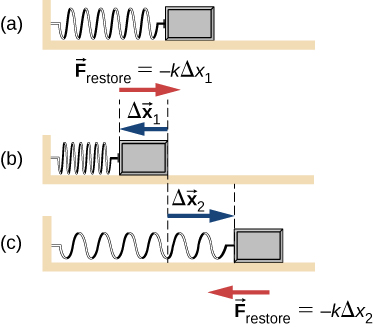
\includegraphics[width=0.33\textwidth]{figures/spring.jpeg}
\caption{\label{fig:1} A spring exerts a force on a mass when compressed or stretched.}
\end{figure}


\end{document}
